\documentclass[a4paper,ngerman]{scrartcl}

\usepackage{amsmath}
\usepackage{amsfonts}
\usepackage{amssymb}
\usepackage[utf8]{inputenc}
\usepackage{graphicx}
\usepackage[ngerman]{babel}
\usepackage{hyperref}
\usepackage{float}
\usepackage{caption}
\usepackage{subcaption}
\usepackage{multirow}  %for tables
\usepackage{icomma} % Handle german comma as decimal point in numbers
\usepackage{units,siunitx} % Write units with correct spacing
\usepackage{upgreek} % provide non-italic greek letters
\usepackage{url}
\usepackage{extpfeil}
%\usepackage{subfig}

% Formatting of table & figure captions
\captionsetup{font={sf,footnotesize},labelfont=bf,textfont=sl,skip=6pt}
\setlength{\abovecaptionskip}{6pt}
\setlength{\belowcaptionskip}{0pt}

\title{Black Lipid Membrane (BLM)\\Vorbereitung}
\date{\today}
\author{Michel Rausch, Michael Eliachevitch}

\begin{document}

\maketitle
\tableofcontents
\newpage

\section{Einleitung}

In diesem Versuch werden Ionenkanäle in planaren Lipidmembranen untersucht. Hierbei wird der Wirkmechanismus des Antibiotikums Gramacidin A untersucht. In einer biologischen Zelle gelangen durch die entstandenen Kanäle Kationen durch die Zellmembran. Die Zelle stirbt aufgrund der Störung ihres elektrochemischen Gradients [\ref{ref:mappe}].

Gramicidin beschreibt eine Gruppe Antibiotika. Dieses ist kommerziell unter Namen wie Angidin\textregistered , Mycolog\textregistered , Topsym\textregistered , oder Neospiron\textregistered  verfügbar. 


\section{Theoretische Grundlagen}

Gramicidin A1 besitzt die Summenformel $C_{99}H_{140}N_{20}O_{17}$. Es kann in der Natur von im Boden lebenden Bakterien beobachtet werden und wird auch synthetisch hergestellt. Mehrere Strukturen sind möglich, wobei Gramicidin A die häufigste ist. Gramicidin S besitzt eine zyklische Struktur und damit einen anderen Wirkmechanismus. In diesem Experiment wird lediglich die Variante A verwendet.

\subsection{Wirkmechanismus}

Es existieren verschiedene Modelle, die beschreiben, wie Gramicidin A in die Zellmembran integriert wird, welche in Abbildung \ref{fig:wirkmechanismus} aufgelistet sind. Auf die chemischen Grundlagen wird nicht im Detail eingegangen.

\begin{figure}[tb!]
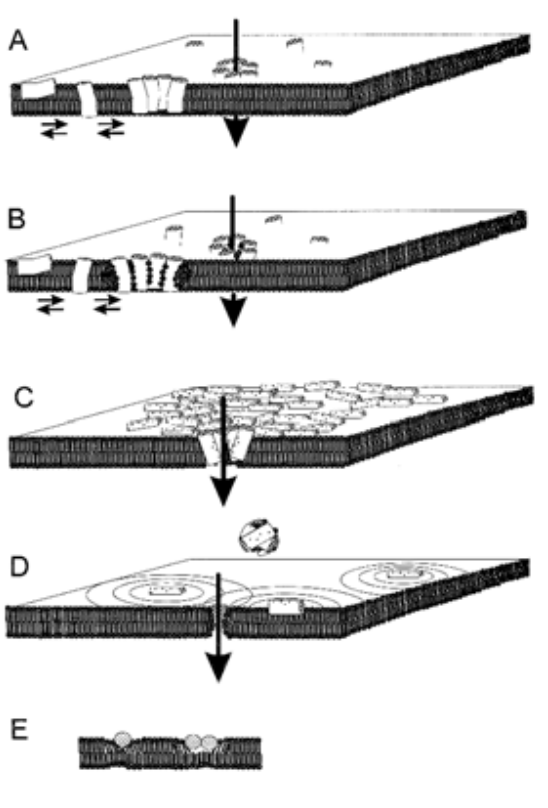
\includegraphics[width=0.5\textwidth]{abbildungen/wirkmechanismus.png}
\caption{\textbf{Verschiedene Modelle zur Erklärung der Zerstörung einer Bakterienzelle mittels Peptid-Antibiotika [\ref{ref:mappe}].}\\
\textbf{A: Barrel Stave model.} 
Hydrophobe, helixförmige Monomere bilden Poren in der Zellmembran. 
Dies ist in BLM-Messung bemerkbar durch schrittweise Erhöhung der Leitfähigkeit.
\textbf{B: Toroidial Wormhole model.}  
Poren werden gebildet in Anwesenheit phosphatidylethanolaminer, oder phosphatidylseriner (PE/PS) Membranen. 
Das führt zu Bindungen zwischen Lipiden und Peptiden.
Zusammen bilden sie die Wände der Poren.
Die Größe der entstandenen Poren variiert.
\textbf{C: Carpet model}  
Teppich-(engl. carpet-) ähnliche Formationen werden auf der Membran gebildet.
Durch eine erhöhte Konzentration dringen mehr Moleküle in die Membran ein und die Lipid-Doppelschicht wird zerstört.
\textbf{D:  Detergent similar model.}
Bi- und Mizellen bilden Flächen auf der Membran, ähnlich dem Mechanismus, der bei Bleichmitteln beobachtet wird.
Durch deren Amphiphilie (Hydrophilie und Lipophilie) werden Bindungen mit Phospholipiden eingegangen.
Die Membran wird durchlässig und die Zelle beschädigt.
\textbf{E:  In-plane diffusion model.}
Die Moleküle können nicht die ganze Schicht bedecken, um Poren zu bilden. 
Sie beeinflussen die Lipidschicht und ihre effektive Dicke nimmt ab.
}
\label{fig:wirkmechanismus}
\end{figure}


\subsection{Ionentransport}

Eine Membran trennt zwei Bereiche einer wässrigen Lösung. Um sie zu überwinden, muss ein Ion eine Energie $E$ aufbringen. Die  Wahrscheinlichkeit k, eines Ions mit der Temperatur T, diese während einer Zeiteinheit zu überwinden ist der Ratenkoeffizient
\begin{equation} \label{eqn:rate}
k = k_0 e^{-\frac{E}{k_B T}},
\end{equation}
mit der Boltzmannkonstante $k_{B}$. Das Potential einer Membran lässt sich wie in Abbildung \ref{fig:potential-einfach} vorstellen. Die Ionen können in der Membran Bindungen eingehen, daher entstehen weitere Minima.

\begin{figure}[tb!]
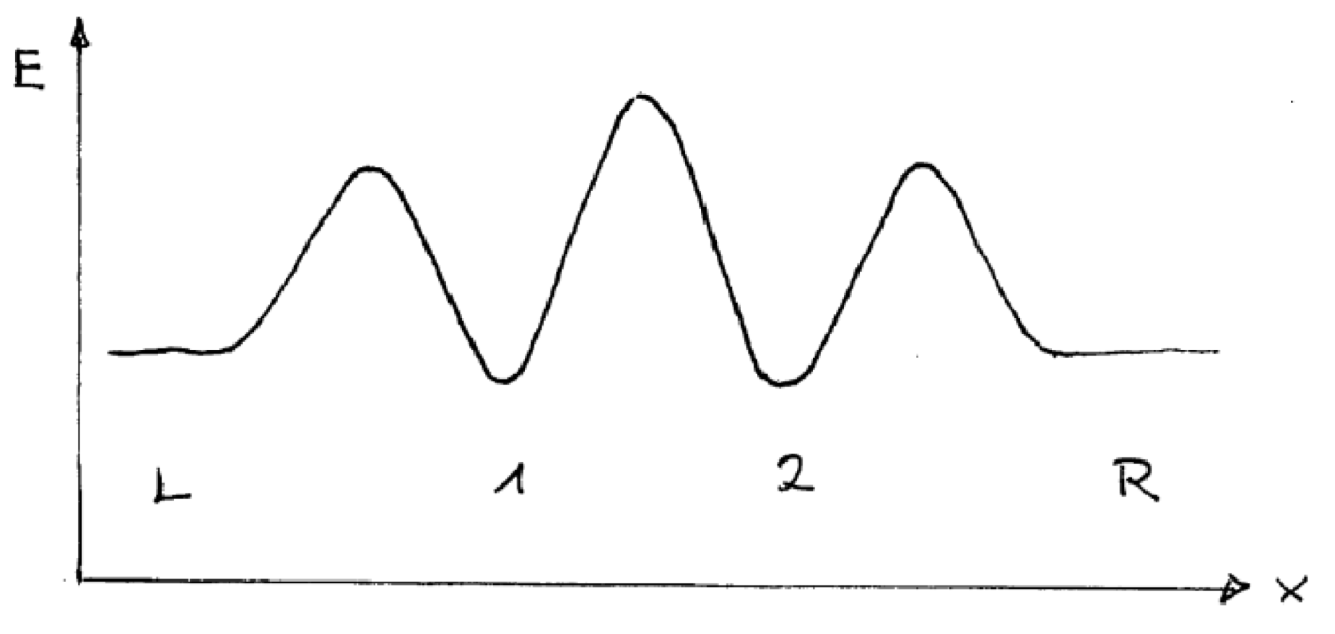
\includegraphics[width=0.6\textwidth]{abbildungen/potential-einfach.png}
\caption{\textbf{Schema eines Potentials einer Pore [\ref{ref:mappe}]}}
\label{fig:potential-einfach}
\end{figure}


Die Gleichung \ref{eqn:rate} wird auf den Fall des Experiments erweitert. Durch die angelegte Spannung $V_{m}$ wird das Potential asymmetrisch, wie in Abbildung \ref{fig:potential-asym} gezeigt.  Es wird die Quasistationaritätsnäherung verwendet. Die Leitfähigkeit eines einzelnen Kanals ist damit

\begin{equation}
\Lambda = \frac{k_A}{k_D} \cdot \frac{c}{k_A^{-1}+k^{-1}+k_D^{-1}} \cdot  \frac{q^2}{k_B T} .
\end{equation}

Mit der Ladung q der Ionen und den Ratenkoeffizienten $k_A$, $k_D$ und $k$ der Membran.
Hieraus ergeben sich die Zusammenhänge der makroskopisch messbaren Größen

\begin{equation}
I_M = \lambda_M \cdot V_m
\end{equation}
und
\begin{equation}\label{eqn:transport-leitfaehigkeit}
\lambda_m = \Lambda \cdot N_p.
\end{equation}

Hierbei ist $I_M$ der gemessene Gesamtstrom durch die Membran und $\lambda_M$ deren Leitfähigkeit.


\begin{figure}[tb!]
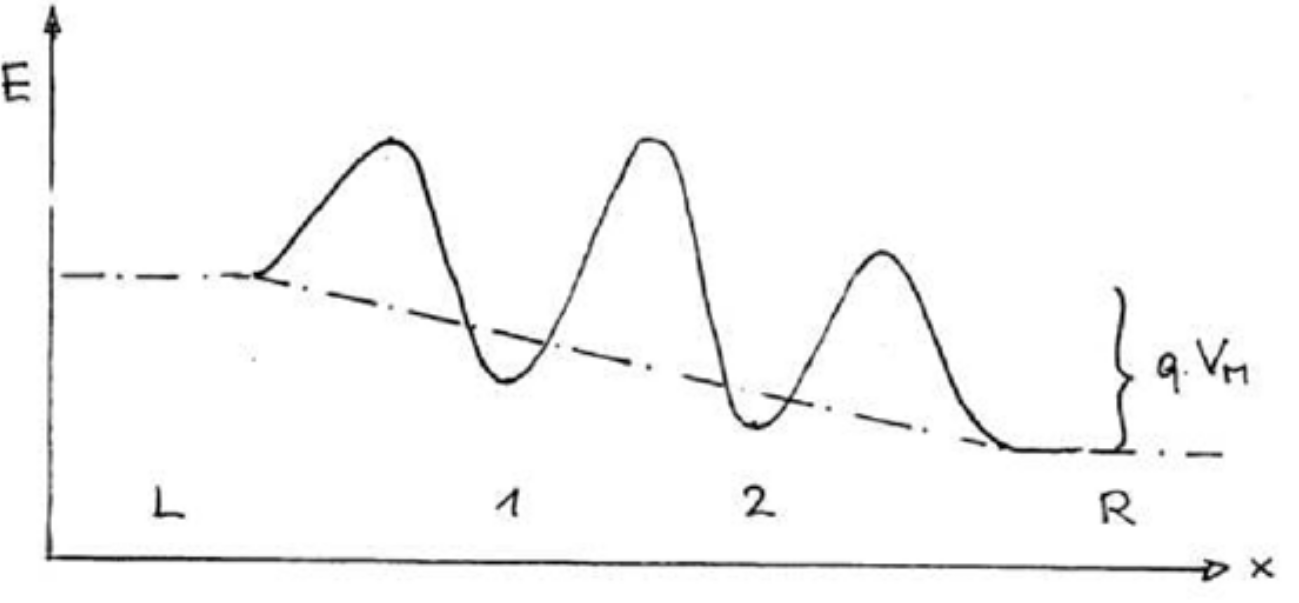
\includegraphics[width=0.6\textwidth]{abbildungen/potential-asym.png}
\caption{\textbf{Schema des Potentials einer Pore mit angelegter Spannung [\ref{ref:mappe}]}}
\label{fig:potential-asym}
\end{figure}



\subsubsection{Einzelkanalentstehung}

Nur Dimere des Gramicidin A führen zu einer Bildung von Ionenkanälen. 
Ist die Rate der Bildung der Dimere gleich der Rate ihrer Vernichtung, spricht man von einem Gleichgewicht.
Ohne äußere Einwirkung bleibt die Zahl der Kanäle etwa gleich.
Die Bildung und Zerstörung sind zufällige Ereignisse, daher kommt es zu einer variierenden Anzahl an Poren in der Membran und somit zu einer Fluktuation der Leitfähigkeit.
Da jeder Kanal gleich zur Leitfähigkeit beiträgt, ist die Gesamtleitfähigkeit quantifiziert. 
Bei einer geringen Konzentration sind nur einzelne Kanäle vorhanden, daher ist die Quantisierung des Stromes $I_M$ deutlich erkennbar.

Die Dimerasation kann durch die Gleichung,

\begin{equation}
G_1 + G_1 	\xtofrom[k_d]{k_r} G_2 ,
\end{equation}

beschrieben werden. $k_d$ ist hier die Rate der Dissoziation und $k_r$ die der Entstehung der Dimere, $G_1$ entspricht den Monomeren, $G_2$ den Dimeren. Die Dissoziation folgt einem exponentiellem Zerfallsgesetz, die der Entstehungsreaktion ist linear zum Quadrat der Konzentration. Aus dem Verlauf des Stromes über die Zeit lässt sich die Zerfallsrate bestimmen.



\subsubsection{Mehrkanalentstehung}

Bei hohen Konzentrationen sind einzelne Kanäle nicht mehr ohne weiteres zu beobachten. Es gibt jedoch ein Rauschen in der Strommessung. Dies entstammt dem Öffnen und schließen von Kanälen. 
Die Reaktionsgleichung ergibt sich als
\begin{equation}\label{eqn:mehrkanal-reaktion1}
\frac{dG_2}{dt} = - k_d \cdot G_2 + k_r \cdot G_1^2 .
\end{equation}
Woraus folgt:
\begin{equation}\label{eqn:mehrkanal-reaktion2}
\frac{G_2}{G_1^2} = \frac{k_r}{k_d} .
\end{equation}

Die Gesamtzahl der Moleküle ist
\begin{equation}
G = G_1 + 2 \cdot G_2.
\end{equation}

Dieser Prozess kann beobachtet werden, wenn das Gleichgewicht, zum Beispiel mit einem elektrischem Feld, oder Temperaturänderung, gestört wird. 
Auch spontane Änderungen der Teilchenzahl sind im Rauschen erkennbar.

Die Relaxationszeit ergibt sich aus Gleichungen \ref{eqn:mehrkanal-reaktion1} und \ref{eqn:mehrkanal-reaktion2}, zusammen mit \ref{eqn:transport-leitfaehigkeit} (mit $G_2 = N_P$) als

\begin{equation}\label{mehrkanal-tau}
\tau^{-1} = k_d + 4 \cdot k_r \cdot G_1 = k_d + 4 \sqrt{\frac{k_d \cdot k_r}{\Lambda}  \cdot \lambda_M} .
\end{equation}

Deutlich zu erkennen ist die inverse wurzelförmige Abhängigkeit zur Leitfähigkeit.

\subsubsection{Autokorrelationsfunktion}

Eine Autokorrelationsfunktion beschreibt die Korrelation eines Signals mit sich selbst zu einem anderen Zeitpunkt. 
Bei einem stochastischem Prozess, wie der Entstehung und Schließung von Kanälen, ist das Zeitprofil der Korrelationsfunktion gleich der Relaxation des Gleichgewichts [\ref{ref:mappe}]. Diese ist in Gleichung \ref{mehrkanal-tau} beschrieben.

Betrachtet man ein ein Signal x(t), welches den Erwartungswert 0 hat, wie das Rauschen des Stroms, so erwartet man, dass der Erwartungswert 

\begin{equation}
<x(t) \cdot x(t+T)> = 0
\end{equation}
für $T \rightarrow \inf $, sowie
\begin{equation}
<x(t) \cdot x(t+T)> = <x^2>
\end{equation}
für $T=0$ ist. 

Die Lebensdauer eines Kanals $\frac{1}{k_d}$ definiert somit die Relaxationszeit.  Es genügt also die Korrelationsfunktion zu analysieren. Die einzelnen Kanäle müssen nicht beobachtet werden und das Rauschen ist reduziert.



\clearpage
\section{Versuchsaufbau und Versuchsdurchführung}



\subsection{Versuchsaufbau und Vorbereitung der Lösungen}
\label{sec:bilayer-vorbereitung}

\begin{figure}[tb!]
  \centering
  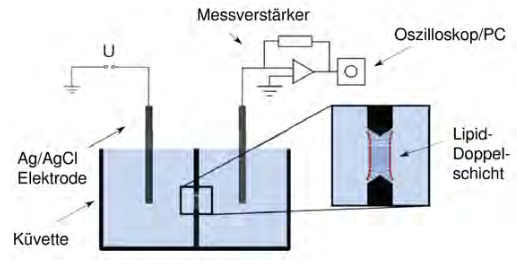
\includegraphics[width=0.8\textwidth]{abbildungen/blmaufbau.png}
  \caption{\textbf{Aufbau einer BLM ("`Black Lipid Membrane"').} \\Eine Küvette ist durch eine hydrophobe Trennwand zweigeteilt. Diese Trennwand hat ein kleines Loch in der Größenordnungen von Mikrometern, auf das eine Lipid-Doppelschicht "`aufgemalt"' wird. Da sie im getrockneten Zustand eine molekulare Dicke von nur einigen Nanometern hat, kommt es zu destruktiver Interferenz des an beiden Seiten reflektierten Lichtes und sie erscheint schwarz, weshalb die Lipid-Doppelschicht als BML bezeichnet wird. Die Küvette enthält eine Elektrolytlösung und zwischen beiden Hälften kann durch Dioden eine Gleich- oder Wechselspannung angelegt werden. Das Ablesen von elektrischen Signalen erfolgt am Oszilloskop, das hinter einen Verstärker geschaltet ist.\\Quelle: [\ref{ref:mappe}]}
  \label{fig:blmaufbau}
\end{figure}

Der typische Aufbau einer BLM ("`Black Lipid Membrane"') ist in Abbildung \ref{fig:blmaufbau} dargestellt und erklärt. \\

In unserem Fall werden als Elektrolytlösung 0.5\,M Kaliumchlorid (KCl) vorbereitet, um genügend Ionen zur Verfügung zustellen, aber auch nicht zu viele, um die Lipid-Doppelschicht nicht zu zerstören. Die Lipidlösung zum Aufmalen der BLM soll eine Konzentration von 
$\SI{3,5}{mg/ml}$ Glyzerin-Monooleat in Tetradekan haben. Zum Erzeugen der Ionenkanäle in der Membran wird das Antibiotikum Gramicidin A verwendet. Dazu wird zuerst eine
Lösung mit einer Konzentration von $\SI{0,1}{mg/ml}$ hergestellt, von der ein Teil nochmal mit Wasser verdünnt wird, um eine Konzentration von
$\SI{4}{ng/ml}$ zu erhalten. \\

Als Serienwiderstand werden $\SI{100}{k\ohm}$ verwendet und als Feedback-Widerstand $\SI{500}{M\ohm}$. Zuerst werden wir eine 
Rechteck-Wechselspannung mit einer Frequenz von 100\,Hz verwenden, die eine Amplitude zwischen 20 und 100\,mV haben soll. \\



\subsection{Erzeugung der Lidid-Doppelschicht und Messung der Membran-Kapazität}
\label{sec:capacity}
Die Küvette wird in die Apparatur eingesetzt und in beide Hälften wird
die KCl Lösung eingefüllt.

Die Lipidlösung wird mit einem Teflonstäbchen auf das gereinigte Loch aufgetragen, wobei darauf geachtet werden sollte, dass es keine Luftblasen gibt.
Dann soll einige Minuten gewartet werden, damit die Lipid-Doppelschicht ausdünnt.
Dabei kann man durch umrühren und abtragen der Lipidlösung mit dem Teflonstäbchen etwas nachhelfen.
Die Schicht wird dabei mit einer Lampe im Abstand
von 30\,cm beleuchtet. Am Anfang sollten in der Reflexion Newtonsche Ringe sichtbar sein. Wenn das nicht der Fall ist, soll mit einem
Teflonstäbchen etwas von der Schicht entfernt werden. Im getrockneten Zustand sollte die Schicht im Objektiv schwarz erscheinen, da es 
an das an der Vorder- und Rückseite der Schicht reflektierte Licht destruktiv interferiert. Außerdem sollten im getrockneten Zustand 
einer Erhöhung der Membran-Kapazität feststellbar sein. Dabei kann die Membran als Plattenkondensator angenommen werden. Die Kapazität $C$
ist dabei eine Funktion der Dicke $d$ und der Fläche $A$ der Membran
\begin{equation}
C = \epsilon_0 \epsilon_r \frac{A}{d}.
\end{equation}1

Die experimentelle Bestimmung der Kapazität erfolgt über die Messung des Relaxationszeit $\tau$ des Membranstroms $I_C$. Die Entladung erfolgt
exponentiell gemäß der Formel

\begin{equation}
  I_C(t) = - \frac{U_0}{R_C} \cdot e^{\frac{t}{\tau}} = - I_0 \cdot e^{\frac{t}{R_C C}},
\end{equation}

wobei $R_C$ den reellen Widerstand des Kondensators bezeichnet. Der Entladevorgang findet immer dann statt, wenn die Rechteckspannung umschwenkt. Die Spannung $U_0$ entspricht dann der doppelten Spannungsamplitude der Spannungsquelle.
Es folgt, dass sich die Kapazität berechnen lässt über

\begin{equation}
  C = \frac{\tau}{R_C}~.
\end{equation}

Die spezifische Kapazität
\begin{equation}
  C_S = \frac{C}{A}
\end{equation}
soll ebenfalls bestimmt werden. 
Sie kennzeichnet das Verhältnis von der Kapazität $C$ zur Membranfläche $A$.
Diese kann näherungsweise bestimmt werden, indem man eine Aufnahme von der Öffnung macht, an der sich die Membran befindet und das Verhältnis der Membranfläche zu der bekannten Fläche der Öffnung geometrisch bestimmt.

\subsection{Messung einzelner Ionenkanäle}
\label{sec:singlechannels}
Die Widerstände werden in diesem Versuchsteil gleich gelassen, aber statt der Wechselspannung wird nun an der Membran eine Gleichspannung 
von 50\,mV verwendet. Es soll eine kleine Menge Gramicidin A hinzugefügt und dabei der Membranstrom aufgezeichnet werden. Da der Strom 
sprunghaft mit der Anzahl der Kanäle steigen sollte, kann durch Differenzbildung an einer Stufe der Strom durch einen einzigen Kanal bestimmt werden. Wenn dieser Strom bekannt ist, kann man folglich immer sehen, wenn ein neuer Kanal entsteht oder zerfällt.\\

Damit kann nun ein Histogramm der Kanal-Lebenszeiten erzeugt werden. Unter der Exponentialverteilung kann damit die mittlere Lebensdauer 
eines Kanals und der Ratenkoeffizient für den Zerfall von Gramicidin A bestimmt werden.

\subsection{Messung multipler Ionenkanäle}
\label{sec:multiplechannels}
Nun soll die Konzentration von Gramicidin A erhöht werden, sodass viele Ionenkanäle entstehen. 
Mithilfe der gegebenen Analyse-Software wird ein Histogramm des Membranstroms erstellt. 
Für die Häufigkeit der vorkommenden Ströme erwartet man, dass sich um den mittleren Membranstrom ein Peak bildet und sich weitere Peaks mit einem diskretem Abstand, der dem Strom durch einen einzelnen Kanal entspricht, bilden.
Daraus sollen die Stufenhöhen und deren Mittelwerte bestimmt werden, was durch Messung der Position der Peaks und der dazugehörigen Stromdifferenz erfolgt.

\subsection{Noise-Analyse und Autokorrelationsfunktion}
\label{sec:noise-autocorr}
Nun soll eine solche Menge von Gramicidin A hinzugefügt werden, dass man mehrere Ionenkanäle erhält, sodass die Grundlinie nicht mehr sichtbar ist und keine Stufen im Strom durch die Membran mehr enthalten sind. 
Durch die Zerstörung und Bildung von Kanälen fluktuiert der Strom etwas um den mittleren Strom.
Nun soll eine Analyse dieses Rauschens mit der Autokorrelationsfunktion durchgeführt werden und
mit den Ergebnissen von dem Lebenszeit-Histogramm aus der Einzelkanalmessung verglichen werden, indem auch hier der Kanalstrom und die Kanal-Lebenszeit bestimmt werden. 
\subsection{Weitere Fragen}
\label{sec:weitere-fragen}

\begin{itemize}
\item Vergleich der Methoden
\item Bestimmung der Einzelkanalleitfähigkeit
\item Bestimmung des Ratenkoeffizienten
\item Berechnung des Partikelstroms durch einen Kanal
\end{itemize}













\section{Quellen}
\begin{enumerate}
\item Vorbereitungsmappe \label{ref:mappe}
\item pharmawiki.ch (16.11.2014) \label{ref:pharmawiki}
\item Zusammenhänge von Struktur und Funktion unterschiedlicher membranaktiver Peptide, Christian Mink,  (2010)
\end{enumerate}



\end{document}
